\documentclass[utf8]{beamer}
\mode<presentation>
\usepackage{listings}
\usepackage{helvet}
\usetheme{Warsaw}
\usecolortheme{whale}
\usefonttheme[onlylarge]{structuresmallcapsserif}
\usefonttheme[onlysmall]{structurebold}
\usepackage{amsthm} % pushQED, popQED
\newenvironment{aquote}[1]{%
  \pushQED{#1}%
  \begin{quote}
}{%
  \par\noindent\hfill(\popQED)%
  \end{quote}%
}

\setbeamercovered{dynamic}
\setbeameroption{show notes}

\begin{document}
\title{Scaling Erlang Web Applications}
\subtitle{100 to 100K users at one web server}
\author{Fernando Benavides (\textit{@elbrujohalcon})}
\institute{Inaka Labs}
\date{\today}
\logo{
\includegraphics[height=0.5cm]{img/inaka_leaf_logo.png}}

\newcommand*\oldmacro{}%
\let\oldmacro\insertshorttitle%
\renewcommand*\insertshorttitle{%
  \oldmacro\hfill%
  \insertframenumber\,/\,\inserttotalframenumber}

%%%%%%%%%%%%%%%%%%%%%%%%%%%%%%%%%%%%%%%%%%%%%%%%%%%%%%%%%%%%%%%%%%%%%%
%% CODE SNIPPETS
%%%%%%%%%%%%%%%%%%%%%%%%%%%%%%%%%%%%%%%%%%%%%%%%%%%%%%%%%%%%%%%%%%%%%%
\definecolor{darkblue}{rgb}{0,0.08,0.45} 

\lstset{% general command to set parameter(s)
		mathescape=true,
		language=erlang,
		basicstyle=\ttfamily\small,
		keywordstyle=\color{blue}\bfseries,
		identifierstyle=\color{darkblue},
		stringstyle=\ttfamily,
		showstringspaces=false}

\defverbatim[colored]\startchild{%
\begin{lstlisting}[frame=single]
start_user(User) ->
  Manager =
    list_to_atom(
      "user-manager-" ++
        integer_to_list($\colorbox{yellow}{\texttt{random:uniform(?MANAGERS)}}$)),
  supervisor:start_child(Manager, [User]).
\end{lstlisting}
}
\defverbatim[colored]\startchildinit{%
\begin{lstlisting}[frame=single]
init([]) ->
  _ = random:seed(erlang:now()),
  Managers =
    [{list_to_atom("user-manager-" ++
                     integer_to_list(I)),
      $\colorbox{yellow}{\texttt{\{user\_mgr, start\_link, [I]\}}}$,
      permanent, brutal_kill, supervisor,
      [user_mgr]}
     || I <- $\colorbox{yellow}{\texttt{lists:seq(1, ?MANAGERS)}}$],
  {ok, {{one_for_one, 5, 10}, Managers}}.
\end{lstlisting}
}

\defverbatim[colored]\backlog{%
\begin{lstlisting}[frame=single]
gen_tcp:listen(Port,
  [binary, {packet, line}, {keepalive, true},
   {active, false}, {reuseaddr, true},
   $\colorbox{yellow}{\texttt{\{backlog, 128000\}}}$, {send_timeout, 32000},
   {send_timeout_close, true}]).
\end{lstlisting}
}
\defverbatim[colored]\backlogweb{%
\begin{lstlisting}[frame=single]
mochiweb_http:start(
  [{name, ?MODULE}, {loop, {?MODULE, loop}},
   $\colorbox{yellow}{\texttt{\{backlog, 128000\}}}$, {port, Port}]).
\end{lstlisting}
}
\defverbatim[colored]\db{%
\begin{lstlisting}[frame=single]
-define(REDIS_CONNECTIONS, 200).
-record(state, {redis :: $\colorbox{yellow}{\texttt{[pid()]}}$}).
$\large \ldots$
Redis =
  lists:map(
    fun(_) ->
      {ok, Conn} = erldis_client:start_link()
      Conn
    end, $\colorbox{yellow}{\texttt{lists:seq(1, ?REDIS\_CONNECTIONS)}}$),
{ok, #state{redis = Redis}}.
\end{lstlisting}
}

\defverbatim[colored]\dbcall{%
\begin{lstlisting}[frame=single]
handle_call(Request, From, State) ->
  $\colorbox{yellow}{\texttt{[RedisConn|Redis] = State\#state.redis}}$,
  proc_lib:spawn_link(
    fun() ->
      Res = handle_call(Request, RedisConn),
      gen_server:reply(From, Res)
    end),
  {noreply, State#state{redis =
                          $\colorbox{yellow}{\texttt{Redis ++ [RedisConn]}}$}}.
\end{lstlisting}
}

\defverbatim[colored]\listener{%
\begin{lstlisting}[frame=single]
init([]) ->
$\large \ldots$
  Listeners =
    [{list_to_atom("client-listener-" ++
                     integer_to_list(I)),
      $\colorbox{yellow}{\texttt{{client\_listener, start\_link, [\textbf{I}]}}}$,
      permanent, brutal_kill, worker,
      [client_listener]}
     || I <- $\colorbox{yellow}{\texttt{lists:seq(MinPort, MaxPort)}}$],
  {ok, {{one_for_one, 5, 10}, Listeners}}.
\end{lstlisting}
}

\defverbatim[colored]\suphandler{%
\begin{lstlisting}[frame=single]
EvtMgr =
  match_stream_match:event_manager(MatchId),
ok =
  gen_event:add_handler(EvtMgr,
    {?MODULE, {MatchId,UserId,Client}}, self()),
$\colorbox{yellow}{\texttt{MgrRef = erlang:monitor(process, EvtMgr)}}$,
ClientRef = erlang:monitor(process, Client),
{reply, ok,
 State#state{matches =
  [{Client, MatchId, ClientRef, MatchRef}
   | State#state.matches]}}
\end{lstlisting}
}
\defverbatim[colored]\suphandlerinfo{%
\begin{lstlisting}[frame=single]
handle_info({'DOWN',Ref,_,Client,_}, State) ->
$\large \ldots$
  case $\colorbox{yellow}{\texttt{lists:keytake(Ref, 4, State\#state.matches)}}$ of
    {value, {Client,_,CRef,Ref}, OtherMatches} ->
      $\large \ldots$
\end{lstlisting}
}

\defverbatim[colored]\repeater{%
\begin{lstlisting}[frame=single]
start_link(Name, Source) ->
  {ok, Pid} = gen_event:start_link(Name),
  ok = gen_event:add_handler(
         Source, {?MODULE, Pid}, Pid),
  {ok, Pid}.
  $\ldots$
init(Repeater) ->
  Ref = erlang:monitor(process, Repeater),
  {ok, #state{mgr = Repeater, ref = Ref}}.
  $\ldots$
handle_event(Event, State) ->
  gen_event:notify(State#state.mgr, Event),
  {ok, State}.
\end{lstlisting}
}

\defverbatim[colored]\reply{%
\begin{lstlisting}[frame=single]
handle_call(Request, From, State) ->
  [RedisConn|Redis] = State#state.redis,
  proc_lib:spawn_link(
    fun() ->
      Res = handle_call(Request, RedisConn),
      $\colorbox{yellow}{\texttt{gen\_server:reply(From, Res)}}$
    end),
  {$\colorbox{yellow}{\texttt{noreply}}$, State#state{redis =
                          Redis ++ [RedisConn]}}.
\end{lstlisting}
}

\defverbatim[colored]\hibernate{%
\begin{lstlisting}[frame=single]
handle_cast(Event, State) ->
  $\large \ldots$
  {noreply, State, $\colorbox{yellow}{\texttt{hibernate}}$}.

$\large \ldots$

handle_call(Request, _From, State) ->
  $\large \ldots$
  {reply, Reply, State, $\colorbox{yellow}{\texttt{hibernate}}$}.
\end{lstlisting}
}

\defverbatim[colored]\init{%
\begin{lstlisting}[frame=single]
init(UserId) ->
  {ok, #state{user = UserId}, $\colorbox{yellow}{\texttt{0}}$}.
  
$\large \ldots$

handle_info($\colorbox{yellow}{\texttt{timeout}}$, State) ->
  case match_stream_db:user(State#state.user) of
  $\large \ldots$
\end{lstlisting}
}

%%%%%%%%%%%%%%%%%%%%%%%%%%%%%%%%%%%%%%%%%%%%%%%%%%%%%%%%%%%%%%%%%%%%%%

\frame{\titlepage} 

\begin{frame}{Hello World!}
	\begin{itemize}
		\item<+-> I'm a developer since I was 10
		\item<+-> I worked with Visual Basic, C\#, .NET, Javascript \ldots
		\item<+-> I switched to functional programming in 2008
		\item<+-> I wrote my thesis project in Haskell
		\item<+-> I'm an Erlang developer since then
	\end{itemize}
\end{frame}
\begin{frame}{Inaka}
	
\end{frame}

\section{Introduction}
\subsection{Description}
\begin{frame}{Introduction}
	My talk is on the scalability of a \emph{web} project \pause that has an \emph{HTTP API} \pause and a component that keeps clients \emph{connected} to the server for \emph{long periods} of time.\\ ~ \\ \pause
	It's a design pattern seen in many places:
	\begin{itemize}
		\item Chat Applications
		\item Social Sites
		\item Sport Sites
	\end{itemize}
\end{frame}

\subsection{Scope}
\begin{frame}{Scope}
	\emph{We will improve the way we use}
	\begin{itemize}
		\item OTP behaviours
		\item TCP and HTTP connections
		\item Underlaying system configurations
	\end{itemize}
	\pause
	\emph{We will \textbf{not} deal with}
	\begin{itemize}
		\item Multiple machines/nodes
		\item Database choices and/or implementations
	\end{itemize}
\end{frame}

\section{Match Stream}
\subsection{Idea}
\begin{frame}[t]{Match Stream}{General Idea}
	\only<1>{
		\emph{A soccer match is played at some stadium}
		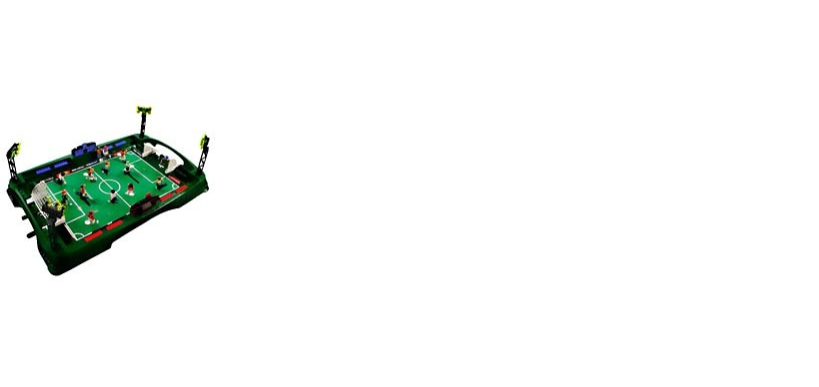
\includegraphics[width=\textwidth]{img/overview-1.png}}
	\only<2>{
		\emph{Soccer fans are connected to the internet in their offices}
		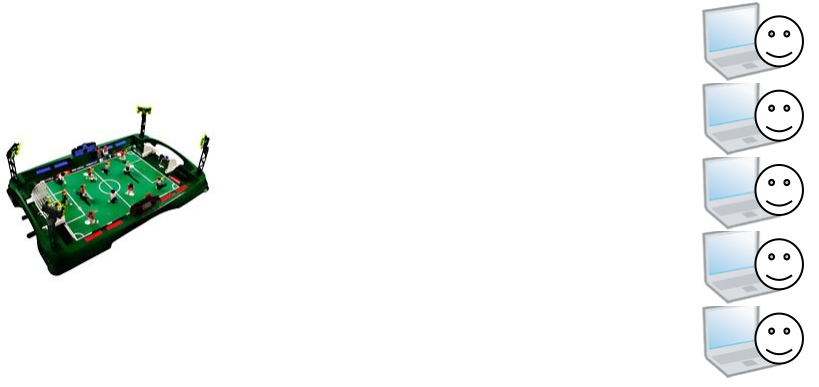
\includegraphics[width=\textwidth]{img/overview-2.png}}
	\only<3>{
		\emph{A reporter is at the stadium with his device}
		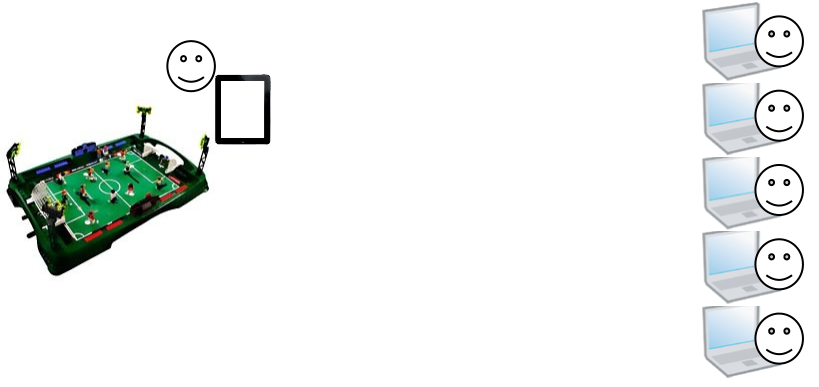
\includegraphics[width=\textwidth]{img/overview-3.png}}
	\only<4>{
		\emph{\textsc{MatchStream} \textbf{connects} them in \textbf{real time}}
		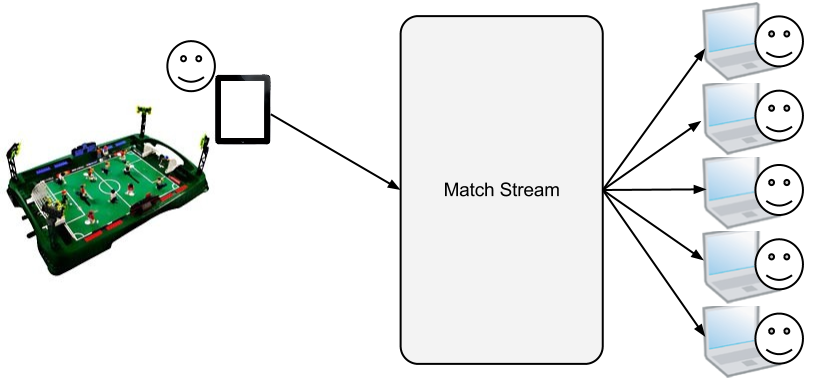
\includegraphics[width=\textwidth]{img/overview-4.png}}
\end{frame}
\begin{frame}{Match Stream}{Requirements}
	\textsc{System Challenges}
	\begin{itemize}
		\item<+-> Many concurrent users connecting at the same time
		\item<+-> Two-hour-long bursts of connections followed by long periods of inactivity
		\item<+-> Real-time updates
	\end{itemize}
	\onslide<+->Erlang seems to be \textbf{the right fit for this}
\end{frame}

\subsection{Design}
\begin{frame}{Match Stream}{General Design}
	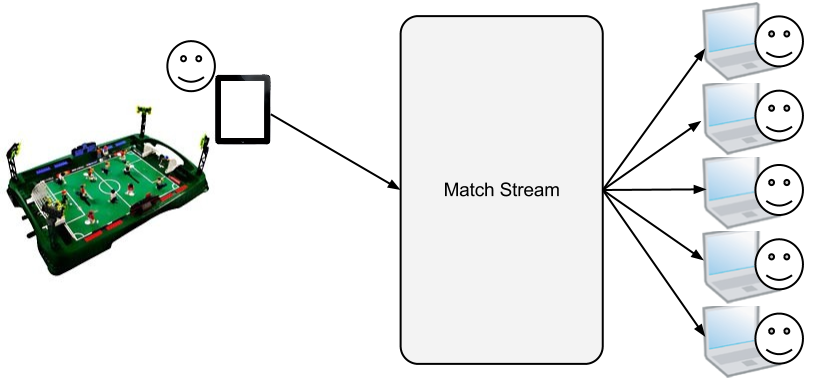
\includegraphics[width=\textwidth]{img/MatchStream.png}
\end{frame}
\begin{frame}[t]{Match Stream}{Architecture}
	\begin{center}
		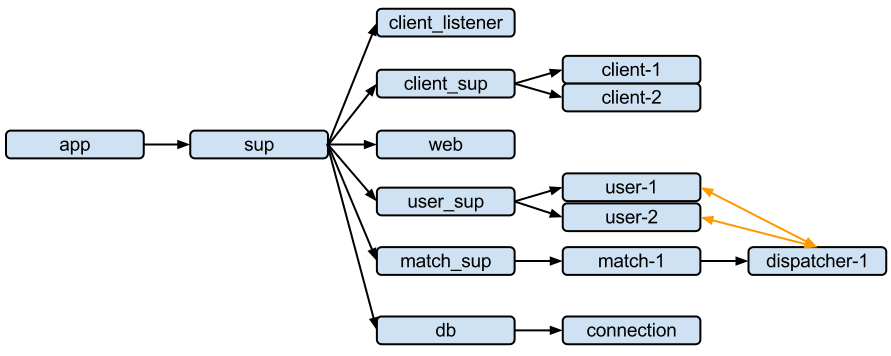
\includegraphics[width=\textwidth]{img/architecture-1.png}
	\end{center}
\end{frame}
\begin{frame}{Components}
	\begin{columns}
		\column{.5\textwidth}
			\only<1>{
				\begin{center}
					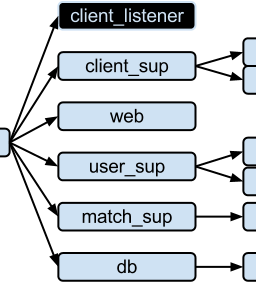
\includegraphics[width=\textwidth]{img/architecture-1-1.png}
				\end{center}}
			\only<2>{
				\begin{center}
					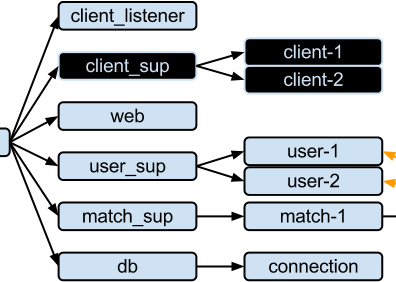
\includegraphics[width=\textwidth]{img/architecture-1-2.png}
				\end{center}}
			\only<3>{
				\begin{center}
					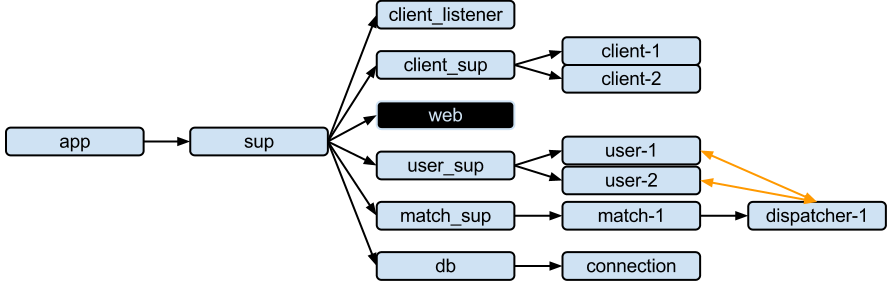
\includegraphics[width=.75\textwidth]{img/architecture-1-3.png}
				\end{center}}
			\only<4>{
				\begin{center}
					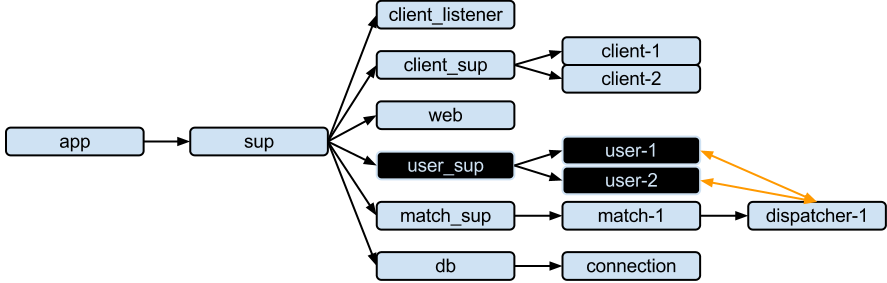
\includegraphics[width=\textwidth]{img/architecture-1-4.png}
				\end{center}}
			\only<5>{
				\begin{center}
					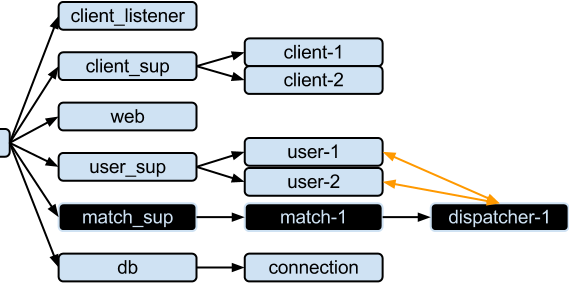
\includegraphics[width=\textwidth]{img/architecture-1-5.png}
				\end{center}}
			\only<6>{
				\begin{center}
					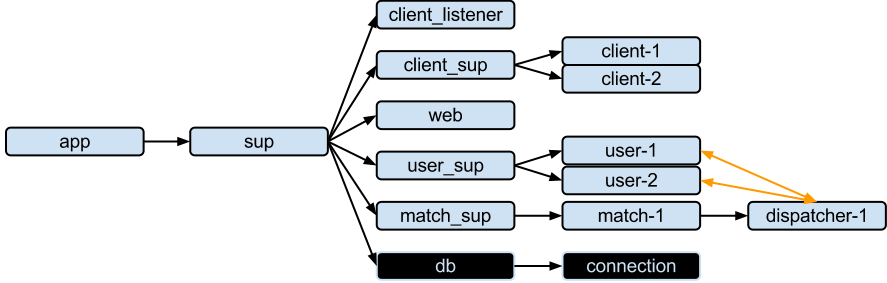
\includegraphics[width=\textwidth]{img/architecture-1-6.png}
				\end{center}}
		\column{.5\textwidth}
			\only<1>{
				\begin{description}
					\item[client\_listener]
						\texttt{gen\_server}. Listens on a TCP port to receive client connections
					\end{description}}
			\only<2>{
				\begin{description}
					\item[client\_sup]
						\texttt{supervisor}. Supervises connection processes
					\item[client]
						\texttt{gen\_fsm}. \\ Handles a TCP connection
				\end{description}}
			\only<3>{
				\begin{description}
					\item[web]
						\texttt{mochiweb server}. Listens for HTTP API calls
				\end{description}}
			\only<4>{
				\begin{description}
					\item[user\_sup]
						\texttt{supervisor}. Supervises user processes
					\item[user]
						\texttt{gen\_server}. Subscribes to match dispatchers and sends events to clients
				\end{description}}
			\only<5>{
				\begin{description}
					\item[match\_sup]
						\texttt{supervisor}. Supervises match processes
					\item[match]
						\texttt{gen\_server}. Listens to match events, stores them
					\item[dispatcher]
						\texttt{gen\_event dispatcher}. Delivers match events
				\end{description}}
			\only<6>{
				\begin{description}
					\item[db]
						\texttt{gen\_server}. Processes database operations
					\item[connection]
						\texttt{erldis client}. Handles the connection to the database
		\end{description}}
	\end{columns}
\end{frame}

\section{Scaling}
\begin{frame}{Lesson Learned}
	\begin{center}
		\huge \emph{Simply using Erlang to build your system is \textbf{not enough} to ensure \textbf{scalability}}
	\end{center}
\end{frame}

\begin{frame}{Measures}
	\begin{description}
		\item[N] \emph{Connections}. Number of connections the server can handle
		\item[C] \emph{Concurrency}. Number of multiple connections starting at a time
		\item[ART] \emph{Average Response Time}. How much does it take for the server to send an event
	\end{description}
\end{frame}
\begin{frame}{Tools}
	\begin{description}
		\item[Test Client]~\\ We create our own test client for TCP connections
		\item[ApacheBench]~\\ To test API calls
		\item[entop]~\\ We use it to see what's going on in the server
	\end{description}
\end{frame}

\subsection{Stage 0: Baseline}
\begin{frame}{Stage 0}{Establishing a Baseline}
	\textsc{Goals}
	\begin{itemize}
		\item Find how much the system can handle
	\end{itemize}
	\pause
	\textsc{Steps}
	\begin{itemize}
		\item Create automated testers
		\item Start the system on a \emph{clean} machine
		\item Test repeatedly adjusting the number of connections
		\item Have a human using the system himself
	\end{itemize}
\end{frame}
\begin{frame}{Stage 1}{Results}
	\begin{columns}
		\column{.66\textwidth}
			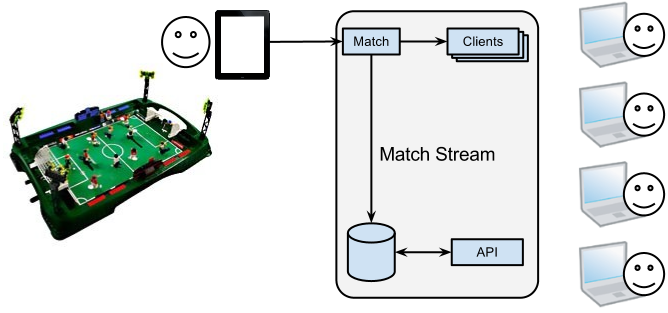
\includegraphics[top=-1,width=\textwidth]{img/results-1.png}
		\column{.33\textwidth}
			\begin{description}
				\item[N] \textbf{\Large 1000}
				\item[C] \textbf{\Large 5}
				\item[ART] \textbf{\Large 26s}
			\end{description}
	\end{columns}
\end{frame}

\subsection{Stage 1: OS Tune}
\begin{frame}{Stage 1}{Tune the OS and the VM}
	\textsc{Goals}
	\begin{itemize}
		\item Improve the underlying Operating System
		\item Improve the Erlang VM Configuration
	\end{itemize}
	\pause
	\textsc{Settings to Tune Up}
	\begin{itemize}
		\item<+-> Open files limit
		\item<+-> TCP connections limit
		\item<+-> TCP backlog size
		\item<+-> TCP memory allocation
		\item<+-> Number of Erlang processes
	\end{itemize}
\end{frame}
\begin{frame}{Stage 1}{Results}
	\begin{columns}
		\column{.66\textwidth}
			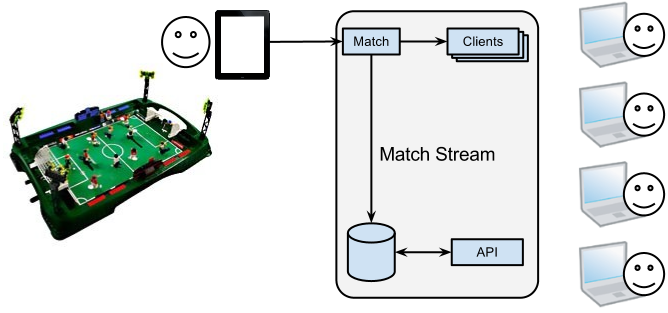
\includegraphics[top=-1,width=\textwidth]{img/results-2.png}
		\column{.33\textwidth}
			\begin{description}
				\item[N] \textbf{\Large 4000}
				\item[C] \textbf{\Large 5}
				\item[ART] \textbf{\Large 35s}
			\end{description}
	\end{columns}
\end{frame}

\subsection{Stage 2: Tune the Code}
\begin{frame}{Stage 2}{Improving Match Stream}
	\begin{center}
		\Large We can't blame the machine anymore, we need to improve \alert{our system}
	\end{center}
\end{frame}

\subsubsection{TCP Tuning}
\begin{frame}{Stage 2.1}{Connection Tweaks}
	\begin{description}
		\item<+->[Backlog]\ \\
			\begin{itemize}
				\item Allow more concurrent connections
				\item Don't forget TCP tuning your HTTP server
			\end{itemize}
	\end{description}
\end{frame}
\begin{frame}{Stage 2.1}{Connection Tweaks}
	\begin{description}
		\item[client\_listener]~\\\backlog
		\item[web]~\\\backlogweb
	\end{description}
\end{frame}
\begin{frame}{Stage 2.1}{Connection Tweaks}
	\begin{description}
		\item<+->[Outbound Connections]\ \\
			\begin{itemize}
				\item For instance, database connections
				\item Don't use just one of them
				\item You may have separated connections for different purposes
			\end{itemize}
	\end{description}
\end{frame}
\begin{frame}{Stage 2.1}{Connection Tweaks}
\only<1>{\db}
\only<2>{\dbcall}
\end{frame}
\begin{frame}{Stage 2.1}{Connection Tweaks}
	\begin{description}
		\item<+->[Listeners]\ \\
			\begin{itemize}
				\item You can listen to more than one port
				\item For unified urls, use \emph{nginx} in front of the server
			\end{itemize}
	\end{description}
\end{frame}
\begin{frame}{Stage 2.1}{Connection Tweaks}
\listener
\end{frame}
\begin{frame}{Stage 2.1}{Connection Tweaks}
	\begin{columns}
		\column{.5\textwidth}
			\begin{center}
				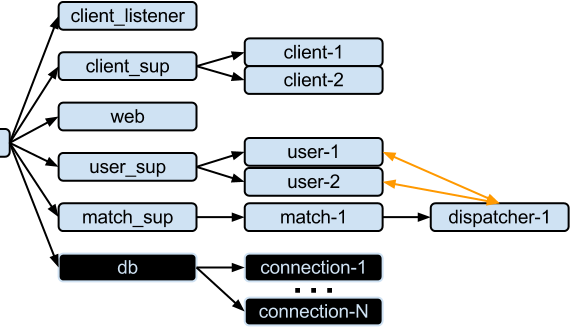
\includegraphics[height=.7\textheight]{img/architecture-2.png}
			\end{center}
		\column{.5\textwidth}
			\begin{description}
				\item[listener]
					\texttt{gen\_server}. Listens on a TCP port to receive client connections
				\item[web]
					\texttt{mochiweb server}. Listens for HTTP API calls on a particular port
				\item[connection]
					\texttt{erldis client}. Handles the connection to the database
			\end{description}
	\end{columns}
\end{frame}
\begin{frame}{Stage 2.1}{Results}
	\begin{columns}
		\column{.66\textwidth}
			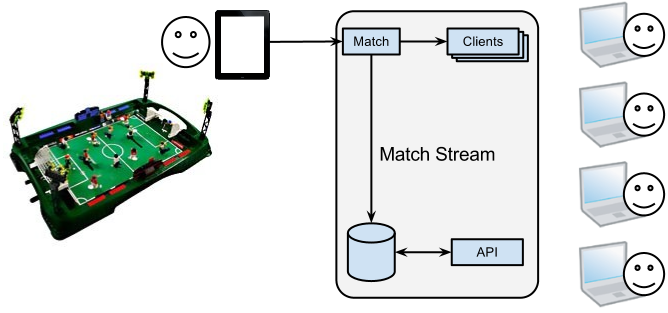
\includegraphics[top=-1,width=\textwidth]{img/results-3-1.png}
		\column{.33\textwidth}
			\begin{description}
				\item[N] \textbf{\Large 8000}
				\item[C] \textbf{\Large 500}
				\item[ART] \textbf{\Large 15s}
			\end{description}
	\end{columns}
\end{frame}

\subsubsection{OTP}
\begin{frame}{Stage 2.2}{gen\textunderscore event}
	\begin{description}
		\item<+->[sup\textunderscore handler]\ \\
			\begin{itemize}
				\item Don't use it
				\item Monitor the processes instead
			\end{itemize}
	\end{description}
\end{frame}
\begin{frame}{Stage 2.2}{gen\textunderscore event}
	\only<1>{\suphandler}
	\only<2>{\suphandlerinfo}
\end{frame}
\begin{frame}{Stage 2.2}{gen\textunderscore event}
	\begin{description}
		\item<+->[Long Delivery Queues]\ \\
			\begin{itemize}
				\item Distribute the work
				\item Use \emph{repeaters}
			\end{itemize}
	\end{description}
\end{frame}
\begin{frame}{Stage 2.2}{gen\textunderscore event}
\repeater
\end{frame}
\begin{frame}{Stage 2.2}{gen\textunderscore event}
	\begin{columns}
		\column{.5\textwidth}
			\begin{center}
				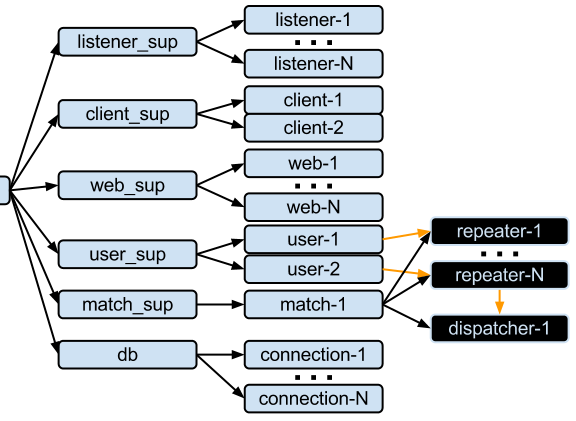
\includegraphics[height=.75\textheight]{img/architecture-3-2.png}
			\end{center}
		\column{.5\textwidth}
			\begin{description}
				\item[repeater]
					\texttt{gen\_event dispatcher}. It's subscribed to \texttt{dispatcher} and \emph{repeats} the received events to its subscribers
			\end{description}
	\end{columns}
\end{frame}
\begin{frame}{Stage 2.2}{Results}
	\begin{columns}
		\column{.66\textwidth}
			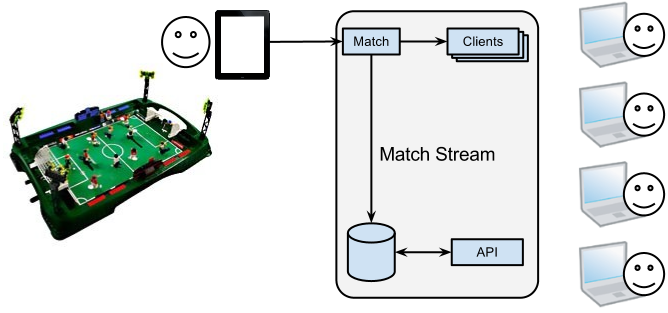
\includegraphics[top=-1,width=\textwidth]{img/results-3-2.png}
		\column{.33\textwidth}
			\begin{itemize}
				\item[N] \textbf{\Large 8000}
				\item[C] \textbf{\Large 500}
				\item[ART] \textbf{\Large 8s}
			\end{itemize}
	\end{columns}
\end{frame}
\begin{frame}{Stage 2.3}{gen\textunderscore server}
	\begin{description}
		\item<+->[Call Timeouts]\ \\
			Remember \texttt{gen\textunderscore server:reply/2}
	\end{description}
\end{frame}
\begin{frame}{Stage 2.3}{gen\textunderscore server}
\reply
\end{frame}
\begin{frame}{Stage 2.3}{gen\textunderscore server}
	\begin{description}
		\item<+->[Memory Footprint]\ \\
			Remember \texttt{hibernate}~\\
	\end{description}
	\begin{aquote}{Erlang Docs}
		Puts the calling process into a wait state where its memory allocation has been reduced as much as possible, which is useful if the process does not expect to receive any messages in the near future.
	\end{aquote}
\end{frame}
\begin{frame}{Stage 2.3}{gen\textunderscore server}
\hibernate
\end{frame}
\begin{frame}{Stage 2.3}{gen\textunderscore server}
	\begin{description}
		\item<+->[Long startup time]\ \\
			\begin{itemize}
				\item Initialize your gen\textunderscore servers in a $0$ timeout
				\item Move initialization code to \texttt{handle\_info}
			\end{itemize}
	\end{description}
\end{frame}
\begin{frame}{Stage 2.3}{gen\textunderscore server}
\init
\end{frame}
\begin{frame}{Stage 2.3}{Results}
	\begin{columns}
		\column{.66\textwidth}
			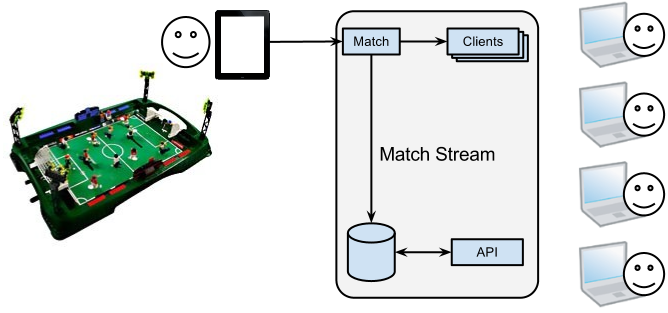
\includegraphics[top=-1,width=\textwidth]{img/results-1.png}
		\column{.33\textwidth}
			\begin{description}
				\item[N] \textbf{\Large 32K}
				\item[C] \textbf{\Large 2000}
				\item[ART] \textbf{\Large 1s}
			\end{description}
	\end{columns}
\end{frame}
\begin{frame}{Stage 2.4}{supervisors}
	\begin{description}
		\item<+->[Simple One for Ones]\ \\
			\begin{itemize}
				\item Sometimes \texttt{simple\textunderscore one\textunderscore for\textunderscore one} supervisors get \alert{overburdened} because they have too many children
				\item Use a supervisor hierarchy
			\end{itemize}
	\end{description}
\end{frame}
\begin{frame}{Stage 2.4}{supervisors}
\only<1>{\startchildinit}
\only<2>{\startchild}
\end{frame}
\begin{frame}{Stage 2.4}{supervisors}
	\begin{columns}
		\column{.5\textwidth}
			\begin{center}
				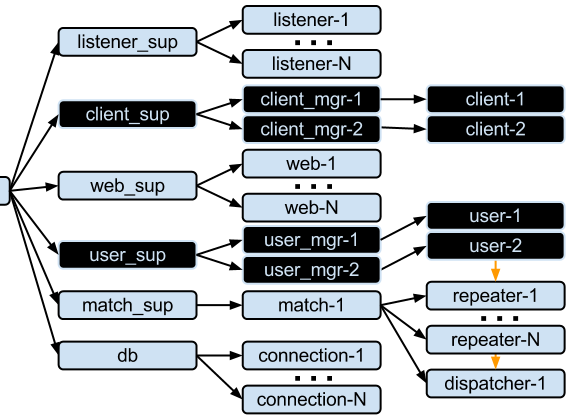
\includegraphics[height=.65\textheight]{img/architecture-3-4.png}
			\end{center}
		\column{.5\textwidth}
			\begin{description}
				\item[user\_mgr]
					\texttt{supervisor}. Supervises a group of users processes
				\item[client\_mgr]
					\texttt{supervisor}. Supervises a group of connection processes
			\end{description}
	\end{columns}
\end{frame}
\begin{frame}{Stage 2.4}{Results}
	\begin{columns}
		\column{.66\textwidth}
			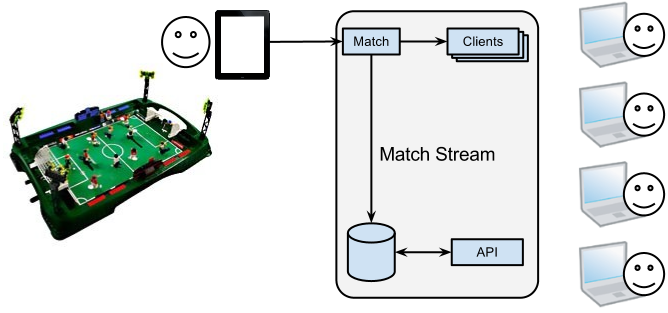
\includegraphics[top=-1,width=\textwidth]{img/results-3-4.png}
		\column{.33\textwidth}
			\begin{itemize}
				\item \textbf{\Large 65536} users
				\item \textbf{\Large 2048} at a time
				\item \textbf{\Large 1s} ART
			\end{itemize}
	\end{columns}
\end{frame}

\subsubsection{Other Stuff}
\begin{frame}{Stage 2.5}{Other Processes}
	\begin{description}
		\item<+->[Logging]\ \\
			\begin{itemize}
				\item Don't log too much
				\item Use a good logging system
			\end{itemize}
		\item<+->[Registration]\ \\
			\begin{itemize}
				\item Sometimes it's better to register processes instead of keeping track of their pids manually
				\item You can always register processes \alert{both} locally and globally
			\end{itemize}
	\end{description}
\end{frame}
\begin{frame}{Stage 2.5}{Other Processes}
	\textsc{System Architecture}
	\begin{center}
		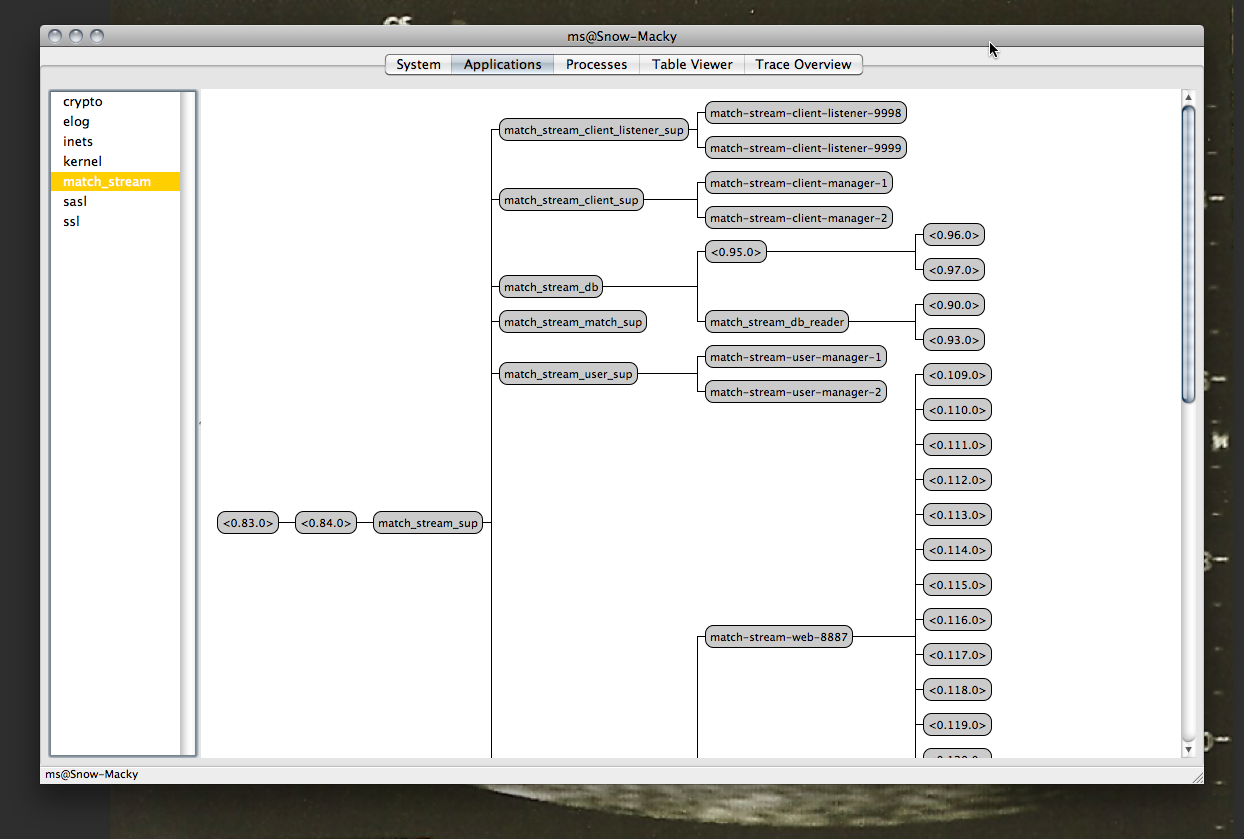
\includegraphics[height=.75\textheight]{img/running-late.png}
	\end{center}
\end{frame}
\begin{frame}{Stage 2.5}{Results}
	\begin{columns}
		\column{.66\textwidth}
			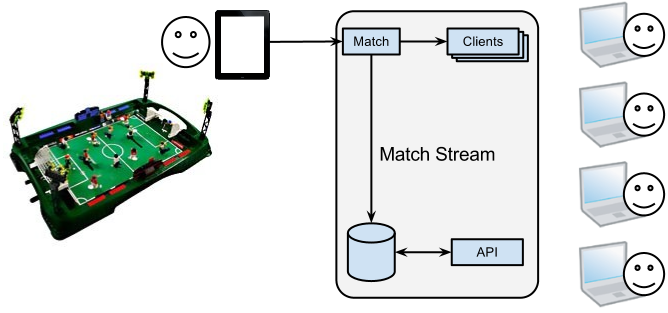
\includegraphics[top=-1,width=\textwidth]{img/results-3-5.png}
		\column{.33\textwidth}
			\begin{itemize}
				\item \textbf{\Large 65536} users
				\item \textbf{\Large 8192} at a time
				\item \textbf{\Large 10ms} ART
			\end{itemize}
	\end{columns}
\end{frame}

\subsection{Stage 3: Multi-Node Tuning}
\begin{frame}{Stage 3}{Adding Nodes}
	\textsc{Goals}
	\begin{itemize}
		\item Find the best system topology
	\end{itemize}
	\pause
	\textsc{Steps}
	\begin{itemize}
		\item Prepare the system to run in more than one node
		\item Decide if nodes should be connected or independent
		\item Decide if nodes should be on the same machine or not
	\end{itemize}
\end{frame}
\begin{frame}{Stage 3}{Adding Nodes}
	\textsc{System Architecture}
	\begin{center}
		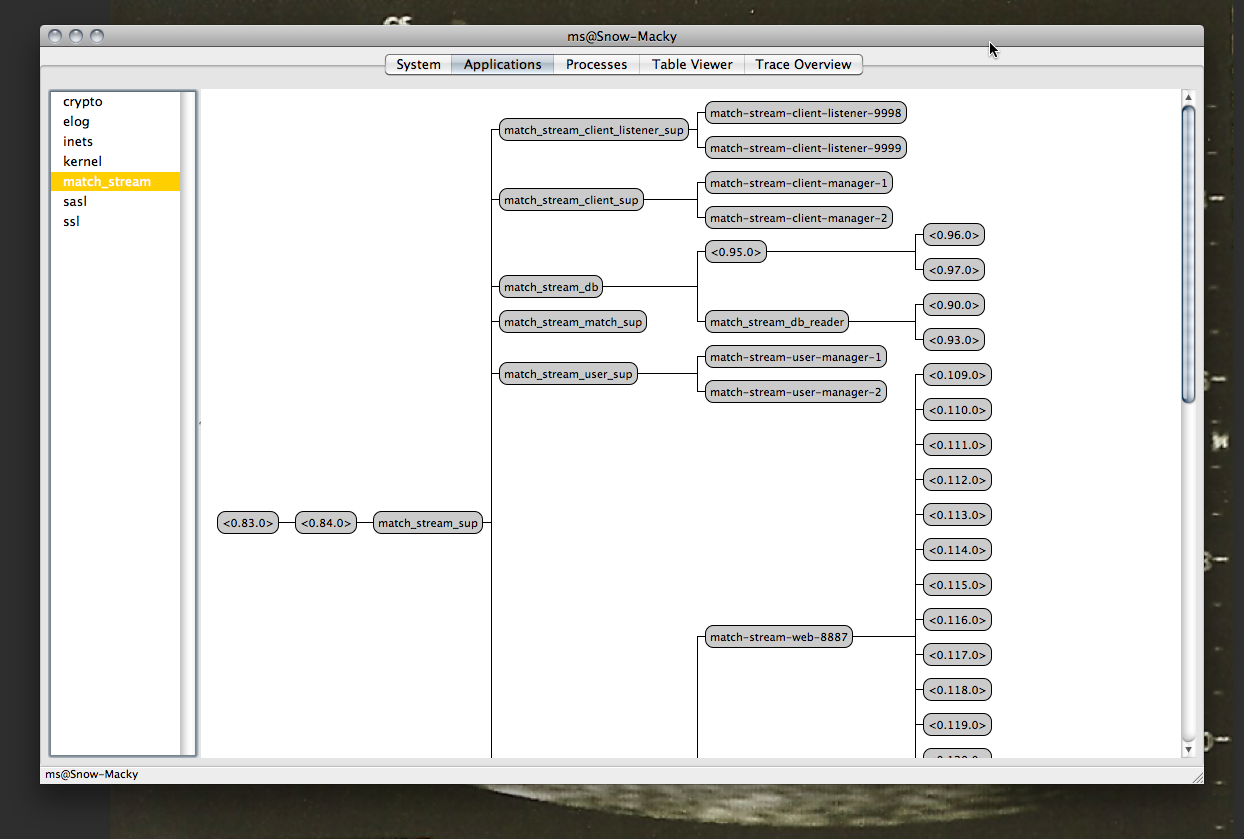
\includegraphics[height=.75\textheight]{img/running-late.png}
	\end{center}
\end{frame}
\begin{frame}{Stage 3}{Results}
	\begin{columns}
		\column{.66\textwidth}
			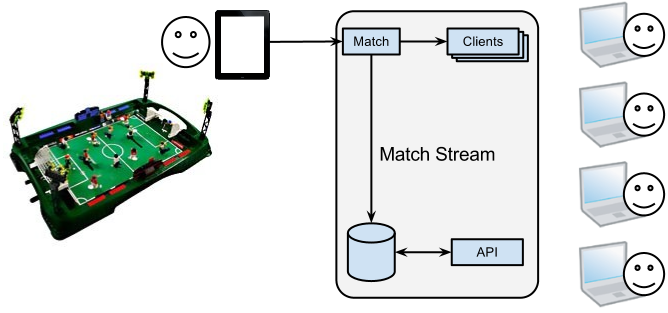
\includegraphics[top=-1,width=\textwidth]{img/results-4.png}
		\column{.33\textwidth}
			\begin{itemize}
				\item \textbf{\Large 100K} users
				\item \textbf{\Large 32768} at a time
				\item \textbf{\Large 10ms} ART
			\end{itemize}
	\end{columns}
\end{frame}

\section{Final Words}
\subsection{Summary}
\begin{frame}{Summary}
	\begin{itemize}
		\item<+-> This is an \alert{iterative} process
		\item<+-> It worked awesomely for us in both experimental and real-life systems
		\item<+-> It's no \alert{silver bullet}
		\item<+-> The list of \emph{Tips and Tricks} grows \alert{constantly} over time
	\end{itemize}
\end{frame}
\subsection{What's next?}
\begin{frame}{Scaling Topics}{that weren't covered on this presentation}
	\begin{itemize}
		\item Managing many nodes
		\item Choosing databases
		\item System specific improvements
		\item Measuring tools
	\end{itemize}
\end{frame}
\subsection{Questions}
\begin{frame}{Questions}
	\begin{center}
		
\includegraphics[width=\textwidth]{img/theriddler.jpg}
	\end{center}
\end{frame}

\appendix

\begin{frame}
	\begin{center}
		{\Huge Thanks!}
	\end{center}
\end{frame}

\end{document}